%%%%%%%%%%%%%%%%%%%%%%%%%
% Dokumentinformationen %
%%%%%%%%%%%%%%%%%%%%%%%%%
% !TeX program = pdflatex
% !TeX encoding = utf8
% !TeX spellcheck = de_DE
\newcommand{\titleinfo}{ElMag - Formelsammlung}
\newcommand{\authorname}{\href{mailto:sreinli@hsr.ch}{S. Reinli} \quad \href{mailto:mgisler@hsr.ch}{M. Gisler} }
\newcommand{\authoremail}{\href{mailto:sreinli@hsr.ch}{sreinli@hsr.ch} \quad \href{mailto:mgisler@hsr.ch}{M. Gisler} }
\newcommand{\versioninfo}{$ Revision: 1.1 $}

%BuG-Fix
%Package pdf Error: Driver file ................ not found
%If you have a luatex driver fail uncomment these lines
\RequirePackage{luatex85}
\def\pgfsysdriver{pgfsys-pdftex.def}

% Genereller Header
\documentclass[11pt,twoside,a4paper,fleqn]{article}
% Dateiencoding
\usepackage[utf8]{inputenc}
\usepackage[T1]{fontenc}	%ä,ü...
% Seitenränder
\usepackage[left=1cm,right=1cm,top=0.5cm,bottom=0.5cm,includeheadfoot]{geometry}
% Sprachpaket
\usepackage[english, ngerman]{babel} % Silbentrennung und Rechtschreibung Englisch und Deutsch

%%%%%%%%%%%%%%%%%%%%%%%
%% Wichtige Packages %%
%%%%%%%%%%%%%%%%%%%%%%%
\usepackage{amsmath}                % Allgemeine Matheumgebungen									
\usepackage{amssymb}                % Fonts: msam,msbm, eufm & Mathesymbole, Mengen (lädt automatisch amsfonts)									
\usepackage{array}                  % \newcolumntype, \firsthline, ,\lasthline, m{width}, b{width}									
\usepackage{caption}                % Bildunterschriften									
\usepackage{enumitem}               % basic environments: enumerate, itemize, description									
\usepackage{fancybox}               % \fbox: \shad­ow­box, \dou­ble­box, \oval­box, \Oval­box									
\usepackage{fancyhdr}               % Seiten schöner gestalten, insbesondere Kopf- und Fußzeile									
\usepackage{floatflt}               % Textumflossene Abbildungen \begin{floatingfigure}[r]{Breite} : r rechts, l links, p links auf geraden Seiten und rechts auf ungeraden Seiten									
\usepackage{graphicx}               % \includegraphics[keyvals]{imagefile}, [draft]graphicx zeigt nur Namen und Rahmen an, [final] hebt diese option auf => Bild wird angezeigt    									
\usepackage{hyperref}               % Erstellt Verweise innerhalb und nach außerhalb eines PDF Dokumentes.									
\usepackage{lastpage}               % Bspw. : Page 1 of 3 => \thepage\ of \pageref{LastPage}									
\usepackage{listings}               % Erlaubt es Programmcode in der gewünschten Sprache zu hinterlegen (C++, Matlab,..). Definition der Sprache mit \lstset{language=name}..									
\usepackage{longtable}              % Longtable erlaubt es Tabellen zu erstellen die bei der nächsten Seite weiterlaufen. (Bricht automatisch um)									
\usepackage{mathabx}                % Mathesymbole									
\usepackage{mathrsfs}               % \mathscr (Benötigt für Fourierreihen-Symbol)									
%\usepackage{mathtools}              % Extension package to amsmath									
\usepackage{multicol}               % multicols-Umgebung \begin{multicols}{3} erzeugt Abschnitt mit 3 Spalten									
\usepackage{multirow}               % Tabelle: ermöglicht es Felder mehrerer Zeilen in einem zusammenzufassen									
\usepackage{pdflscape}              % adds PDF support to the environment 'landscape'									
\usepackage{pxfonts}                % Symbole, griechisches Alphabet, Integrale...									
\usepackage{rotating}               % sideways, turn{degree}, rotate{degree}, sidewaysfigure, sidewaystable Umgebung									
\usepackage{subcaption}             % Bildunterschriften für Subfigures									
\usepackage{tabularx}               % tabularx-Umgebung: Hat feste Gesamtbreite, \begin{tabularx}{\textwidth}{c c c c c} X: Spalte mit variabler Breite, l, c, r, p{breite}, m{breite}									
\usepackage{textcomp}               % text symbols: baht, bullet, copyright, musical-note, onequarter, section, yen									
\usepackage{tikz}                   % Tikz Umgebung zur Grafikerzeugung									
\usepackage{titlesec}               % Überschriften zu Textabstände
\usepackage{trfsigns}               % Transformationszeichen \laplace, \Laplace..									
\usepackage{trsym}                  % Weitere Laplace Zeichen erlaubt auch vertikale Transformationszeichen									
\usepackage{verbatim}               % verbatim, verbatim*, comment Umgebung									
\usepackage{wrapfig}                % Textumflossene Bilder und Tabellen, \begin{wrapfigure}[Zeilen]{Position}[Ueberhang]{Breite}									
\usepackage{xcolor}                 % \pagecolor{color}, \textcolor{color}{text}, \colorbox{color}{text}, \fcolorbox{border-color}{fill-color}{text}									
\usepackage{titlesec}
% Zum Bilder einfach in Tabellen einfügen (valign=t)
\usepackage[export]{adjustbox}

%%%%%%%%%%%%%%%%%%%%
% Generelle Makros %
%%%%%%%%%%%%%%%%%%%%
\newcommand{\skript}[1]{$_{\textcolor{red}{\mbox{\small{Skript S.#1}}}}$}
\newcommand{\verweis}[2]{\small{(siehe auch \ref{#1}, #2 (S. \pageref{#1}))}}
\newcommand{\verweiskurz}[1]{(\small{siehe \ref{#1}\normalsize)}}
\newcommand{\subsubadd}[1]{\textcolor{black}{\mbox{#1}}}
\newcommand{\formelbuch}[1]{$_{\textcolor{red}{\mbox{\small{S#1}}}}$}

\newcommand{\kuchling}[1]{$_{\textcolor{red}{\mbox{\small{Kuchling #1}}}}$}
\newcommand{\stoecker}[1]{$_{\textcolor{grey}{\mbox{\small{Stöcker #1}}}}$}
\newcommand{\sachs}[1]{$_{\textcolor{blue}{\mbox{\small{Sachs S. #1}}}}$}
\newcommand{\hartl}[1]{$_{\textcolor{green}{\mbox{\small{Hartl S. #1}}}}$}

\newcommand{\schaum}[1]{\tiny Schaum S. #1}

\newcommand{\skriptsection}[2]{\section{#1 {\tiny Skript S. #2}}}
\newcommand{\skriptsubsection}[2]{\subsection{#1 {\tiny Skript S. #2}}}
\newcommand{\skriptsubsubsection}[2]{\subsubsection{#1 {\tiny Skript S. #2}}}

\newcommand{\matlab}[1]{\footnotesize{(Matlab: \texttt{#1})}\normalsize{}}

% Syntax: \bmu{Pfad zum Bild}{Bildgrösse}{Beschriftung des Bildes}
\newcommand{\bl}[2]{
	\begin{figure}[h]
		\flushleft  % linksbuendig
		\includegraphics[width=#1]{#2} \\
	\end{figure}
}
\newcommand{\br}[2]{
	\begin{figure}[h]
		\flushright  % rechtsbuendig
		\includegraphics[width=#1]{#2} \\
	\end{figure}
}

\newcommand{\bild}[2]{
	\begin{figure}[h]
		\centering  % zentriert
		\includegraphics[width=#1]{#2} \\
	\end{figure}
}

\newcommand\tabbild[2][]{%
	\raisebox{0pt}[\dimexpr\totalheight+\dp\strutbox\relax][\dp\strutbox]{%
		\includegraphics[#1]{#2}%
	}%
}

\newcolumntype{P}[1]{>{\raggedright\arraybackslash}p{#1}} %Tabelle linksausgerichtet
\newcolumntype{L}[1]{>{\raggedleft\arraybackslash}p{#1}} %Tabelle rechtsausgerichtet
\newcolumntype{C}[1]{>{\centering\arraybackslash}p{#1}}



%%%%%%%%%%
% Farben %
%%%%%%%%%%
\definecolor{black}{rgb}{0,0,0}
\definecolor{red}{rgb}{1,0,0}
\definecolor{white}{rgb}{1,1,1}
\definecolor{grey}{rgb}{0.8,0.8,0.8}
\definecolor{green}{rgb}{0,.8,0.05}
\definecolor{brown}{rgb}{0.603,0,0}
\definecolor{mymauve}{rgb}{0.58,0,0.82}


%%%%%%%%%%%%%%%%%%%%%%%%%%%%
% Mathematische Operatoren %
%%%%%%%%%%%%%%%%%%%%%%%%%%%%
\DeclareMathOperator{\sinc}{sinc}
\DeclareMathOperator{\sgn}{sgn}
\DeclareMathOperator{\Real}{Re}
\DeclareMathOperator{\Imag}{Im}
%\DeclareMathOperator{\e}{e}
\DeclareMathOperator{\cov}{cov}
\DeclareMathOperator{\PolyGrad}{PolyGrad}

%Grösse Integral anpassen
\def\Int{\mbox{\Large$\displaystyle\int$\normalsize}}
\def\OInt{\mbox{\Large$\displaystyle\oint$\normalsize}}

%Makro für 'd' von Integral- und Differentialgleichungen 
\newcommand*{\diff}{\mathop{}\!\mathrm{d}}

%%%%%%%%%%%%%%%%%%%%%%%%%%%
% Fouriertransformationen %
%%%%%%%%%%%%%%%%%%%%%%%%%%%

% Fouriertransformationen
\unitlength1cm
\newcommand{\FT}
{
	\begin{picture}(1,0.5)
	\put(0.2,0.1){\circle{0.14}}\put(0.27,0.1){\line(1,0){0.5}}\put(0.77,0.1){\circle*{0.14}}
	\end{picture}
}


\newcommand{\IFT}
{
	\begin{picture}(1,0.5)
	\put(0.2,0.1){\circle*{0.14}}\put(0.27,0.1){\line(1,0){0.45}}\put(0.77,0.1){\circle{0.14}}
	\end{picture}
}


%%%%%%%%%%%%%%%%%%%%%%%%%%%%
% Allgemeine Einstellungen %
%%%%%%%%%%%%%%%%%%%%%%%%%%%%

%Pdf Info
\hypersetup{pdfauthor={\authorname},pdftitle={\titleinfo},colorlinks=false}
\author{\authorname}
\title{\titleinfo}

% Abstände Text zu Übertiteln / Einzug
\titlespacing{\section}{12pt}{1em}{0.5em}
\titlespacing{\subsection}{12pt}{1em}{0.5em}
\titlespacing{\subsubsection}{12pt}{1em}{0.5em}

%%%%%%%%%%%%%%%%%%%%%%%
% Kopf- und Fusszeile %
%%%%%%%%%%%%%%%%%%%%%%%
\pagestyle{fancy}
\fancyhf{}
%Linien oben und unten
\renewcommand{\headrulewidth}{0.5pt} 
\renewcommand{\footrulewidth}{0.5pt}

%Kopfzeile links bzw innen
\fancyhead[L]{\titleinfo{ }\tiny{(\versioninfo)}}
%Kopfzeile mitte
%\fancyhead[C]{}
%Kopfzeile rechts bzw. aussen
\fancyhead[R]{Seite \thepage { }von \pageref{LastPage}}

%Fusszeile links bzw. innen
\fancyfoot[L]{\footnotesize{\authorname}}
%Fusszeile mitte
%\fancyfoot[C]{\footnotesize{\authoremail}}
%Fusszeile rechts bzw. ausen
\fancyfoot[R]{\footnotesize{\today}}
% Einrücken verhindern versuchen
\setlength{\parindent}{0pt}

%%%%%%%%%%%%%%%%%%%%%%%%%%%%%%%%%%%%%%%
%% Makros & anderer Low-Level bastel %%
%%%%%%%%%%%%%%%%%%%%%%%%%%%%%%%%%%%%%%%
% Zeilenhöhe Tabellen:
\newcommand{\arraystretchOriginal}{1.5}
\renewcommand{\arraystretch}{\arraystretchOriginal}

\makeatletter
%% Makros für den Arraystretch (bei uns meist in Tabellen genutzt, welche Formeln enthalten)
% Default Value
\def\@ArrayStretchDefault{1} % Entspricht der Voreinstellung von Latex

% Setzt einen neuen Wert für den arraystretch
\newcommand{\setArrayStretch}[1]{\renewcommand{\arraystretch}{#1}}

% Setzt den arraystretch zurück auf den default wert
\newcommand{\resetArrayStretch}{\renewcommand{\arraystretch}{\@ArrayStretchDefault}}

% Makro zum setzten des Default arraystretch. Kann nur in der Präambel verwendet werden.
\newcommand{\setDefaultArrayStretch}[1]{%
    \AtBeginDocument{%
        \def\@ArrayStretchDefault{#1}
        \renewcommand{\arraystretch}{#1}
    }
}
\makeatother

%% Achtung Symbol \danger
\newcommand*{\TakeFourierOrnament}[1]{{%
        \fontencoding{U}\fontfamily{futs}\selectfont\char#1}}
\newcommand*{\danger}{\TakeFourierOrnament{66}}
\renewcommand{\familydefault}{\sfdefault}
\normalfont
%%%%%%%%%%%%%%%%%%%%%%%%%%%%%%%%%%%%%%%%%%%%%%%%%%%%%%%%%%%%%%%%%%%%%%%%%%%%%%%%%%%%%%%%%%%%%%%%
%TdM Taschenbuch der Mathematik Bronstein
%9., korrigierte Auflage
%iSBN 978-3-8085-5671-9

%%%%%%%%%%%%%%%%%%%%%%%%%%%%%%%%%%%%%%%%%%%%%%%%%%%%%%%%%%%%%%%%%%%%%%%%%%%%%%%%%%%%%%%%%%%%%%%%

\begin{document}
%\thispagestyle{empty}
\setcounter{page}{0} %Set PageNumber to 0
{\huge README }
\section*{Beschreibung}
Formelsammlung für Angewandter Elektromagnetismus Felder und Wellen auf Grundlage der Vorlesung HS 16 von Prof. Dr.Jasmin Smajic \newline
Bei Korrekturen oder Ergänzungen wendet euch an einen der Mitwirkenden.

\section*{Modulschlussprüfung}
Prüfungsstoff ist der gesamte ElMag-Vorlesungsinhalt des HS2016 einschliesslich aller UE.\newline
Als Hilfsmittel für die Modulschlussprüfung sind die Vorlesungen,\newline
UE-Aufgaben und eigenen Aufzeichnungen sowie der Taschenrechner erlaubt.

\subsection*{Plan und Lerninhalte}
{\scriptsize 
\begin{itemize}
    \item Simulationsbasiertes Design und virtuelles Prototyping 
	\item Dielektrisches Design (die elektrostatischen Gleichungen und Randbedingungen)
	\item Elektromechanisches Design (die magnetostatischen Gleichungen und Randbedingungen,  magnetische Kräfte und ihre Kopplung mit der mechanischen Analyse)
	\item Elektrothermisches Design (Eisen- und Kupferverluste und ihre Kopplung mit der thermischen Analyse)
	\item Elektrodynamische Analyse und dazu gehörende Eigenwertprobleme (Maxwell-Gleichungen, Wellenausbreitung, Wellenleiter, Antennen, Resonatoren und Lichtleitfasern) 
	\item Finite-Element-Methode für elektromagnetische Simulationen 
	\item Skalar-FEM (Elektrostatik, Magnetostatik, Wirbelstromanalyse usw.) 
	\item Vektor-FEM (3-D-Wirbelstromanalyse, Wellenausbreitung, Eigenwertprobleme)
	Praktische Anwendungen 
	\item Dielektrische Berechnungen von Hochspannungsgeräten
	\item Wirbelstromanalyse von Leistungstransformatoren
	\item Elektromagnetische Analyse elektrischer Maschinen
	\item Eigenwertanalyse von Wellenleitern und/oder optischen Leitfasern
\item Elektromagnetische Analyse von Mikrowellen- und/oder optischen Antennen
	\item Elektromagnetische Verträglichkeit (EMV).
\end{itemize}
}
\vfill
\section*{Contributors}
\begin{tabular}{ll}
    Stefan Reinli & stefan.reinli@hsr.ch \\ 
    Michel Gisler& michel.gisler@hsr.ch \\ 
\end{tabular} 

{\scriptsize 
\section*{License}
\textbf{Creative Commons BY-NC-SA 3.0}

Sie dürfen:
\begin{itemize}
    \item Das Werk bzw. den Inhalt vervielfältigen, verbreiten und öffentlich
    zugänglich machen.
    \item Abwandlungen und Bearbeitungen des Werkes bzw. Inhaltes anfertigen.
\end{itemize}
Zu den folgenden Bedingungen:
\begin{itemize}
    \item Namensnennung: Sie müssen den Namen des Autors/Rechteinhabers in der von ihm
    festgelegten Weise nennen.
    \item Keine kommerzielle Nutzung: Dieses Werk bzw. dieser Inhalt darf nicht für
    kommerzielle Zwecke verwendet werden.
    \item  Weitergabe unter gleichen Bedingungen: Wenn Sie das lizenzierte Werk bzw. den
    lizenzierten Inhalt bearbeiten oder in anderer Weise erkennbar als Grundlage
    für eigenes Schaffen verwenden, dürfen Sie die daraufhin neu entstandenen
    Werke bzw. Inhalte nur unter Verwendung von Lizenzbedingungen weitergeben,
    die mit denen dieses Lizenzvertrages identisch oder vergleichbar sind.
\end{itemize}
Weitere Details: http://creativecommons.org/licenses/by-nc-sa/3.0/ch/
}
%If we meet some day, 
%and you think this stuff is worth it, you can buy me a beer in return.
\clearpage
\pagenumbering{arabic}% Arabic page numbers (and reset to 1)
\maketitle
\clearpage
%\vspace{-2.5cm}
\setcounter{tocdepth}{2}
\footnotesize
\tableofcontents
\thispagestyle{empty}
\normalsize
\clearpage
\section{Mathematische Grundlagen}
\subsection{Vektorfelder}
\subsubsection{Divergenz}
	Die Divergenz beschreibt die Quellendichte eines Skalarfeldes. 
	Interpretiert man ein Vektorfeld als Strömungsfeld, so gibt die Divergenz für jede
	Stelle die Tendenz an, ob ein Teilchen in der Nähe zu diesem Punkt hin- bzw.
	von diesem Punkt wegfliesst. Es sagt damit aus, ob und wo das Vektorfeld Quellen
	(Divergenz grösser als Null) oder Senken (Divergenz kleiner als Null) hat. Ist
	die Divergenz überall gleich Null, so bezeichnet man das Feld als quellenfrei.\\
	
	$\boxed{\divergenz \vec{F}=\nabla \cdot \vec{F}= \frac{\partial F}{\partial x}+\frac{\partial F}{\partial y}+\frac{\partial F}{\partial z}}$

\subsubsection{Rotation}
Interpretiert man ein Vektorfeld als Strömungsfeld, so gibt die Rotation für jeden
Ort an, wie schnell und um welche Achse ein mitschwimmender Körper rotieren
würde. Ein Vektorfeld, dessen Rotation überall null ist, nennt man wirbelfrei.\\

$\boxed{\rotation(\vec F)=\nabla\times\vec{F} = 
	\begin{pmatrix}
	(F_3)_y - (F_2)_z\\
	(F_1)_z - (F_3)_x\\
	(F_2)_x - (F_1)_y
	\end{pmatrix} = \left({\frac {\partial F_{z}}{\partial y}}-{\frac {\partial F_{y}}{\partial z}}\right){\hat {e}}_{x}+\left({\frac {\partial F_{x}}{\partial z}}-{\frac {\partial F_{z}}{\partial x}}\right){\hat {e}}_{y}+\left({\frac {\partial F_{y}}{\partial x}}-{\frac {\partial F_{x}}{\partial y}}\right){\hat {e}}_{z} \quad 
	\det
	\begin{vmatrix}
	e_x & e_y&e_z\\
	\dfrac{\partial}{\partial x} & \dfrac{\partial}{\partial x}& \dfrac{\partial}{\partial x}\\
	F_x& F_y & F_z
	\end{vmatrix}}$

\subsubsection{Gradient}
Der Gradient zeigt in einem Vektorfeld immer in die Richtung des steilsten Anstiegs. \\

$\boxed{\gradient(f)= \nabla \cdot f= 	
	\begin{pmatrix}
	\frac{\partial f}{\partial x}\\
	\frac{\partial f}{\partial y}\\
	\frac{\partial f}{\partial z}
	\end{pmatrix} ={\frac {\partial f}{\partial x}}{\hat {e}}_{x}+{\frac {\partial f}{\partial y}}{\hat {e}}_{y}+{\frac {\partial f}{\partial z}}{\hat {e}}_{z} }$

\subsubsection{Vektorpotential}
Das Vektorpotential A(r) ist eine Hilfsgrösse um den Umgang mit der magnetischen Flussdichte B(r) zu vereinfachen. \\
	$\boxed{\begin{matrix}
		B=\mu H\\
		B=\rotation A\\
		\varphi=\oint\limits_{C}A dr
		\end{matrix}}$

\subsubsection{Vektorfeldoperatoren}
\begin{tabular}{ll}
	\textbf{Nabla-Operator $\nabla$} & \textbf{Laplace-Operator $\Delta$}\\
	Operator um kontextabhängig & Operator um einem Skalarfeld\\
	Divergenz, Rotation oder Gradient darzustellen  &  die Divergenz seines Gradienten zuzuordnen\\
	$\nabla F=\frac{\partial F}{\partial x}+\frac{\partial F}{\partial y}+\frac{\partial F}{\partial z}$&$\Delta F=\frac{\partial^{2}F}{\partial x^{2}F}+\frac{\partial^{2}F}{\partial y^{2}}+\frac{\partial^{2}}{\partial z^{2}}$\\
	&$\Delta \vec{F} = \divergenz(\gradient(\vec{F}))$\\
	&$\Delta \vec{F} = \nabla \cdot (\nabla \cdot \vec{F})$\\	 
\end{tabular}
\subsubsection{Rechenregeln}
\begin{itemize}
	\item $\rotation(\gradient f) = 0 \qquad $ ``Gradientenfeld ist wirbelfrei''
	\item $\divergenz(\rotation \vec{v}) = 0 \qquad $ ``Feld der Rotation ist quellenfrei''
	\item $\divergenz(f\vec{v}) = (\gradient f) \cdot \vec{v} + f \divergenz \vec{v}$
	\item $\rotation(f\vec{v}) = (\gradient f) \times \vec{v} + f \rotation \vec{v}$
	\item $\rotation(\rotation \vec{v}) = \gradient(\divergenz \vec{v}) - \Delta \vec{v}$
\end{itemize}
\subsubsection{Laplace-Operator Koordinatentranfsormation}
\begin{itemize}
	\item Laplace-Operator in kartesischen Koordinaten
	\[\Delta U(x,y,z) = \frac{\partial^{2}}{\partial x^{2}}+\frac{\partial^{2}}{\partial y^{2}}+\frac{\partial^{2}}{\partial z^{2}}\]
	\item Laplace-Operator in Zylinderkoordinaten
	\[\Delta U(\rho,\varphi,z) = \frac{1}{\rho} \dfrac{\partial}{\partial \rho} \left(\rho \frac{\partial U}{\partial \rho}\right) + \frac{1}{r^2}\frac{\partial^2 U}{\partial \varphi^2}+\dfrac{\partial^2 U}{\partial z^2} \]
	\item Laplace-Operator in Kugelkoordinaten
	\[\Delta U(r,\vartheta,\varphi) = \frac{1}{r^2} \dfrac{\partial}{\partial r} \left( r^2 \frac{\partial U}{\partial r}\right) + \frac{1}{r^2 \sin(\vartheta)}\frac{\partial}{\partial \vartheta}\left(sin(\vartheta)\dfrac{\partial U}{\partial \vartheta} \right) +\frac{1}{r^2 sin^2(\vartheta)}\dfrac{\partial^2 U}{\partial \varphi^2}\]
\end{itemize}
\subsection{Differentialrechnung}
\subsubsection{Ableitungsregeln}
\renewcommand{\arraystretch}{1.5}
\begin{tabular}{|l|l|}
	\hline \textbf{Konstantenregeln}& $c'=0'$\\
	\hline \textbf{Faktorenregeln}& $(cu)'=c u'$\\
	\hline \textbf{Summenregel}& $(u\pm v)'= u' \pm v'$\\
	\hline \textbf{Produktregel}& $(uv)'=u'v + uv'$\\
	\hline \textbf{Quotientenregel}& $(\frac{u}{v})'= \frac{u'v-uv'}{u^{2}}$\\
	\hline \textbf{Kettenregel}& $y=u(v(x)) ; y'=\frac{du}{dv} \frac{dv}{dx}$\\
	\hline \textbf{Potenzregel} & $(u^{a})'=au^{a-1}$\\
	& $(\frac{1}{u})'= \frac{u'}{u^2}$\\
	\hline	\textbf{Wurzelregel} & $f(x)=\sqrt{x} ; f'(x)=\frac{1}{2\sqrt{x}}$\\
	\hline	\textbf{Logarithmusregel} & $\ln{u}'=\frac{u'}{u}$\\ 
	\hline	\textbf{Differentation der Umkehrfunktion} & $(f^{-1})'(y)=\frac{1}{f'(x)} $\\
	\hline 
\end{tabular}
\subsubsection{Ableitung elementarer Funktionen}
\renewcommand{\arraystretch}{2.2}
\begin{tabular}{|l|l||l|l|}
	\hline
	\textbf{Funktion} & \textbf{Ableitung} & \textbf{Funktion} &
	\textbf{Ableitung}\\\hline
	\hline $C$ (Konstante) & 0 & $\sec x$ & $\dfrac{\sin x}{\cos^2 x}$ \\
	\hline $x$ & 1 & $\sec^{-1} x$ & $\dfrac{-\cos x}{\sin^2 x}$\\
	\hline $x^n$ ($n\in\mathbb{R}$) & $nx^{n-1}$ & $\arcsin x \quad (|x| < 1)$ &
	$\dfrac{1}{\sqrt{1-x^2}}$\\
	\hline $\dfrac{1}{x}$ & $-\dfrac{1}{x^2}$ & $\arccos x \quad (|x| < 1)$ &
	$-\dfrac{1}{\sqrt{1-x^2}}$\\
	\hline $\dfrac{1}{x^n}$ & $-\dfrac{n}{x^{n+1}}$ & $\arctan x$ & $\dfrac{1}{1+x^2}$\\
	\hline $\sqrt{x}$ & $\dfrac{1}{2\sqrt{x}}$ & $\arccot{x} $ & $-\dfrac{1}{1+x^2}$\\
	\hline $\sqrt[n]{x}\quad (n\in\mathbb{R}, n \neq 0, x > 0)$ &
	$\dfrac{1}{n\sqrt[n]{x^{n-1}}}$ & $\arcsec x$ & $\dfrac{1}{x\sqrt{x^2-1}}$\\
	\hline $\mathrm{e}^x$ & $\mathrm{e}^x$ & $\arcossec x$ & $-\dfrac{1}{x\sqrt{x^2-1}}$\\
	\hline $\mathrm{e}^{bx}\quad (b\in\mathbb{R})$ & $b\mathrm{e}^{bx}$ & $\sinh x$ &
	$\cosh x$\\
	\hline $a^x\quad (a > 0)$ & $a^x\ln a$ & $\cosh x$ & $\sinh x$\\
	\hline $a^{bx}\quad (b\in\mathbb{R}, a > 0)$ & $ba^{bx}\ln a$ & $\tanh x$ &
	$\dfrac{1}{\cosh^2 x}$\\
	\hline $\ln x$ & $\dfrac{1}{x}$ & $\coth x \quad(x \neq 0)$ & $-\dfrac{1}{\sinh^2 x}$\\
	\hline $\log_a{x} \quad (a > 0, a \neq 1, x > 0)$ &
	$\dfrac{1}{x}\log_a{\mathrm{e}}=\dfrac{1}{x\ln a}$ & $\arsinh x$ &
	$\dfrac{1}{\sqrt{1+x^2}}$\\
	\hline $\lg x \quad (x > 0)$ & $\dfrac{1}{x}\lg \mathrm{e}\approx \dfrac{0.4343}{x}$
	& $\arcosh x \quad (x > 1)$ & $\dfrac{1}{\sqrt{x^2-1}}$\\
	\hline $\sin x$ & $\cos x$ & $\artanh x \quad (|x| < 1)$ & $\dfrac{1}{1-x^2}$\\
	\hline $\cos x$ & $-\sin x$ & $\arcoth x \quad (|x| > 1)$ & $-\dfrac{1}{x^2-1}$\\
	\hline $\tan x \quad (x\neq(2k+1)\dfrac{\pi}{2}, k\in\mathbb{Z})$ & $\dfrac{1}{\cos^2
		x}=\sec^2 x$ & $[f(x)]^n \quad (n\in\mathbb{R})$ & $n[f(x)]^{n-1}f'(x)$\\
	\hline $\cot x \quad (x\neq k\pi, k\in\mathbb{Z})$ & $\dfrac{-1}{\sin^2 x}=-cosec^2x$ & $\ln f(x) \quad (f(x)> 0)$ & $\dfrac{f'(x)}{f(x)}$\\
	\hline
\end{tabular}
\clearpage
\pagebreak
\subsection{Lineare Differentialgleichung 2. Ordnung}
\renewcommand{\arraystretch}{1.2}
\begin{tabular}{p{8cm}p{8cm}}
	\textbf{Form:} $y''+a_1\cdot y'+a_0\cdot y=f(x)$  &
	\textbf{St"orglied:} $f(x)$\\
	\textbf{Homogene Differentialgleichung:} $f(x)=0$ &
	\textbf{Inhomogene Differentialgleichung:} $f(x)\neq 0$\\
	\textbf{Allgemeine Lösung einer DGL: }	$Y=y_H+y_P$& \\
\end{tabular}

\subsubsection{Homogene Lösung $y_H$}
\begin{tabular}{p{8cm}p{8cm}}
	\textbf{Charakteristisches Polynom:}\newline
	$\lambda^2+a_1\cdot\lambda+a_0=0$&	
	\textbf{Durch Mitternachtsformel lösen: }\newline
	$\lambda_{1,2}={\frac {-b\pm {\sqrt {b^{2}-4ac}}}{2a}}$\\\\
	
\end{tabular}

\begin{tabular}{|p{6cm}|p{8cm}|}
	\hline
	Falls $ \lambda_1\neq \lambda_2$&
	$y_H=A_1e^{\lambda_1x}+A_2e^{\lambda_2x}$\\
	\hline
	Falls $\lambda_1= \lambda_2$&
	$y_H=e^{\lambda_1x}(A_1+A_2\cdot x)$\\
	\hline
	Falls $\lambda_{1,2}= -\frac{a_1}{2} \pm jb$&
	$y_H=e^{-\frac{1}{2}a_1x}(A \cdot cos(b) +B \cdot sin(b))$\\
	\hline
\end{tabular}

\subsubsection{Partikuläre Lösung $y_P$ durch Form des Störglieds $f(x)$}
\textbf{Allgemeines Vorgehen:}\\
1. Ermitteltes $y_P$ n mal ableiten \\
2. Ableitungen in DGL einsetzen \\
3. Koeffizientenvergleich \\
\vspace{0.2cm}\\
\begin{tabular}{|p{8cm}|p{10cm}|}
	\hline 	
	Störglied $g(x)$ & Ansatz $y_p$ \\
	\hline
	$k$ (Konstante) & $A$ \\
	\hline
	$x^n$ & \multirow{2}{*}{$A_n*x^n + \dots + A_1*x + A_0$} \\
	$p_n(x) = b_n*x^n + \dots + b_1*x + b_0$ & \\
	\hline
	$k*e^{m*x}$ & $A*e^{m*x}$ \\
	\hline	
	$k*cos(b*x)$ & \multirow{3}{*}{$A*cos(b*x) + B*sin(b*x)$} \\
	$k*sin(b*x)$ & \\
	$k_1*cos(b*x) + k_2*sin(b*x)$ & \\
	\hline
	$k*e^{m*x}*cos(b*x)$ & \multirow{3}{*}{$e^{m*x}*(A*cos(b*x) + B*sin(b*x))$} \\
	$k*e^{m*x}*sin(b*x)$ & \\
	$e^{m*x}*(k_1*cos(b*x) + k_2*sin(b*x)$ & \\
	\hline
	$k*cosh(b*x)$ & \multirow{3}{*}{$A*cosh(b*x) + B*sinh(b*x)$} \\
	$k*sinh(b*x)$ & \\
	$k_1*cosh(b*x) + k_2*sinh(b*x)$ & \\
	\hline
	$k*e^{m*x}*cosh(b*x)$ & \multirow{3}{*}{$e^{m*x}*(A*cosh(b*x) + B*sinh(b*x))$} \\
	$k*e^{m*x}*sinh(b*x)$ & \\
	$e^{m*x}*(k_1*cosh(b*x) + k_2*sinh(b*x)$ & \\
	\hline
	$k*x*e^{mx}$ & $(A*x+B)*e^{m*x}$ \\
	\hline
	$p_n(x)*e^{m*x}$ & $(A_n*x^n + \dots + A_1*x + A_0)*e^{mx}$ \\
	\hline
	$x*(k_1*cos(b*x) + k_2*sin(b*x))$ & $(A_1*x+B_1)*cos(b*x) + (A_2*x+B_2)*sin(b*x)$ \\
	\hline
	$x*e^{mx}*(k_1*cos(b*x) + k_2*sin(b*x))$ & $e^{mx}*((A_1*x+B_1)*cos(b*x) + (A_2*x+B_2)*sin(b*x))$ \\
	\hline
	$x*(k_1*cosh(b*x) + k_2*sinh(b*x))$ & $(A_1*x+B_1)*cosh(b*x) + (A_2*x+B_2)*sinh(b*x)$ \\
	\hline
	$x*e^{mx}*(k_1*cosh(b*x) + k_2*sinh(b*x))$ & $e^{mx}*((A_1*x+B_1)*cosh(b*x) + (A_2*x+B_2)*sinh(b*x))$ \\
	\hline
\end{tabular}
%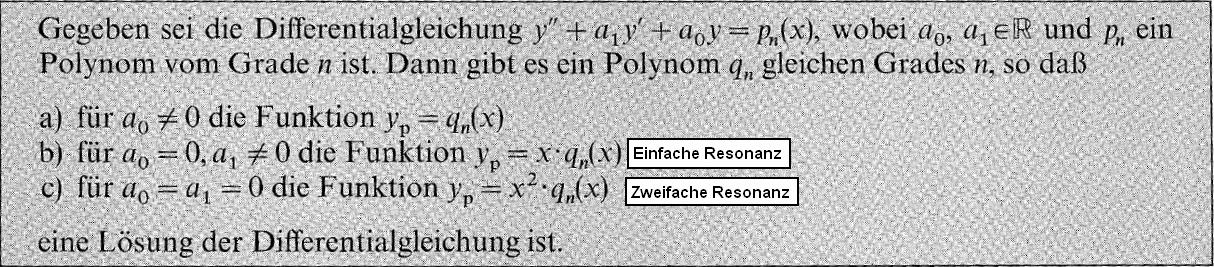
\includegraphics[width=\linewidth]{images/DGL_Part_1.jpg}
%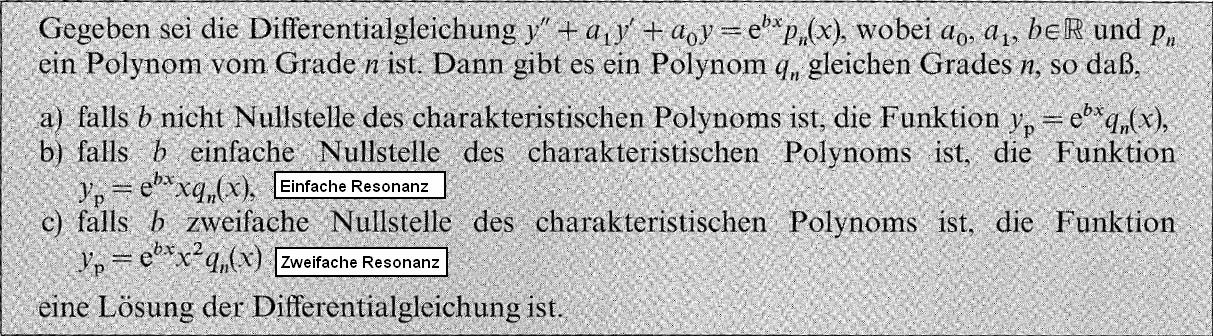
\includegraphics[width=\linewidth]{images/DGL_Part_2.jpg}
%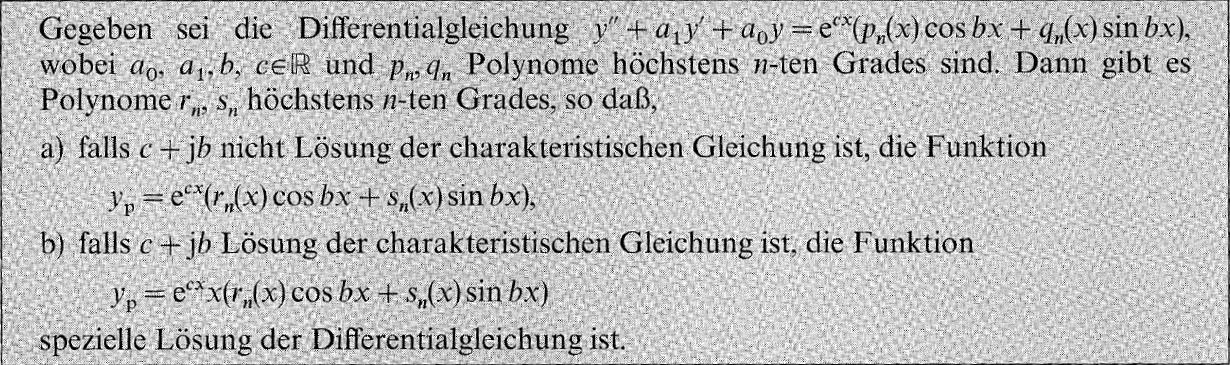
\includegraphics[width=\linewidth]{images/DGL_Part_3.jpg}
\clearpage
\pagebreak

\subsection{Integralgesetze}
\subsubsection{Der Satz von Gauss}
Das Volumenintegral über die Divergenz eines Vektorfeldes wird in ein Oberflächenintegral umgewandelt.\\
$\boxed{\int\limits_V \divergenz \vec F dv = \oint\limits_{\partial V} \vec F \cdot \vec{dA}}$
\subsubsection{Der Satz von Stokes}
Das Oberflächenintegral über die Rotation eines Vektorfeldes wird in ein Kurvenintegral umgewandelt. \\
$\boxed{\int\limits_A \rotation \vec{F}\cdot d\vec{A}  = \oint\limits_{\partial A}\vec{F}\cdot d\vec{s}}$
\subsubsection{Der Satz von Green}
Die Greensche Formel beschreibt den Zusammenhang zwischen Wegintegral und einem Oberflächenintegral.\\
$\boxed{\int\limits_A \frac{\partial F_2}{\partial x} - \frac{\partial F_1}{\partial y} dA = \oint\limits_{\partial A}\vec{F}\cdot d\vec{s}}$
\subsection{Weiteres}
Die Bedeutung der nachfolgenden Integralgleichungen ist die fundamentale Grundlage elektromagnetische Feldtheorie. Der elektrische Strom erzeugt das elektrische Feld in seiner Umgebung (Gausssches Gesetz), der elektrische Strom erzeugt das quellenfreie rotationssymmetrische magnetische Feld (Coulombsches Gesetz), die Verteilung des magnetischen Feldes durch eine geschlossene Kurve ist der gesamte Strom durch die entsprechende Fläche (Ampèresches Gesetz) und das zeitvariante magnetische Feld induziert eine elektrische Spannung (Faradaysches Gesetz).\\
Durch die Gesetze von Stokes und Gauss können diese 4 Gesetze in die Maxwellgleichungen überführt werden. 
\vspace{-0.8cm}
\begin{longtable}{p{.30\textwidth} p{.65\textwidth}}
	\textbf{Elektrostatik} & Die Elektrostatik befasst sich mit ruhenden elektrischen Ladungen, Ladungsverteilungen und den elektrischen Feldern geladener Körper
	Die Phänomene der Elektrostatik rühren von den Kräften her, die elektrische Ladungen aufeinander ausüben. Diese Kräfte werden vom coulombschen Gesetz beschrieben.\\
	\textbf{Elektrodynamik} & Die Elektrodynamik befasst sich mit bewegten elektrischen Ladungen und mit zeitlich veränderlichen elektrischen und magnetischen Feldern. Diese Vorgänge werden durch die Maxwellgleichungen beschrieben. \\
\end{longtable}
\subsection{Einheiten}
\renewcommand{\arraystretch}{1.5}
\begin{tabular}{|p{3.5cm}|p{1.5cm}|p{3cm}||p{3.5cm}|p{1.5cm}|p{3.2cm}|}
	\hline
	\textbf{Name}			&\textbf{Zeichen} & \textbf{Einheit}&
	\textbf{Name}			&\textbf{Zeichen} & \textbf{Einheit}\\
	\hline
	\textbf{Elektr. Feld} 	& $\vec{E}$	& $[E] = \frac{V}{m}$&	
	\textbf{Magn. Feld}		& $\vec{H}$ & $[H] = \frac{A}{m}$\\
	\hline
	\textbf{Elektr. Flussdichte}&$\vec{D}$&$[D] = \frac{C}{m^2}$&
	\textbf{Magn. Flussdichte}&$\vec{B}$&$[B] = \frac{Vs}{m^2}=T$\\
	\hline
	\textbf{Elektr. Stromdichte} &$\vec{J}$& $[J]=\frac{A}{m^2}$&
	\textbf{Elektr. Widerstand} &$R$ &$[R]=\Omega$\\
	\hline
	\textbf{Spannung}&$U$&$[U]=V$&
	\textbf{Strom}&$I$&$[I]=A$\\
	\hline
	\textbf{Induktivität}&$L$&$[L]=\frac{Vs}{A}=H$&
	\textbf{Magn. Spannung}&$V_{m}=\Theta$&$[V_{m}]=A$\\
	\hline
	\textbf{Kapazität}&$C$&$[C]=F$&
	\textbf{Magn. Fluss}&$\phi$&$[\phi]=Wb=Vs$\\
	\hline
	\textbf{Energie}&$W$&$[W]=J=Ws$&
	\textbf{Ladung}&$Q$&$[Q]=C=As$\\
	\hline	
	\textbf{Permeabilität}&$\mu_{0} $&$[\mu_{0}]=4\pi 10^{-7}$&
	\textbf{Permittivität}&$\epsilon_{0}$&$[\epsilon_{0}]=8.854\cdot 10^{-12}$\\
	\hline
	\textbf{Spez. Leitfähigkeit}&$\sigma$&$[\sigma]=\frac{S}{m}$&
	\textbf{Spez. Widerstand}&$\rho $&$[\rho]=\Omega m $\\
	\hline
\end{tabular}

\clearpage
\pagebreak
\section{Elektrostatische Analyse (ES, Electrostatic Analysis)}
Die elektrostatische Analyse arbeitet mit dem elektrostatischen (ruhenden) Feld. In diesem Fall ist die elektrische Ladung stationär verteilt (Ladungsverteilung ändert sich nicht). Mittels dieser Analyse kann das elektrische Feld, die Kapazität und die Energie in den elektrischen Komponenten berechnet werden.
\subsection{Integralgleichungen}
\begin{tabular}{|p{.30\textwidth} |p{.65\textwidth}|}
	\hline
	\textbf{Gausssches Gesetz}\newline
	{\centering\tabbild[width=4cm]{images/Gauss.png}\par}&
	Der Fluss des Vektors $\vec{D} = \varepsilon\cdot\vec{E}$ durch eine geschlossene orientierte Fläche (A) ist gleich der gesamten elektrischen Ladung Q, die von der Fläche (A) umgeben ist.\newline
	\[\varoiint\limits_{(A)}\vec{D}\cdot\vec{dA} = Q \quad oder \quad \varoiint\limits_{(A)}\vec{E}\cdot\vec{dA} = \dfrac{Q}{\varepsilon}\]
	\\
	\hline
	\textbf{Wirbelfreiheit des elektrostatischen Feldes}\newline
	{\centering\tabbild[width=4cm]{images/Wirbelfreiheit}\par}& Das Kurvenintegral des elektrostatischen Feldes $\vec{E}$ über jede geschlossene orientierte Kurve (C) ist gleich null. Das heisst das Kurvenintegral des elektrische Feldes ist nur von der Position des Anfangs- und Endpunkt abhängig. \newline 
	\[\oint\limits_{(C)}\vec{E}\cdot\vec{dl} = 0\] 
	\[\oint\limits_{(C)}\vec{E}\cdot\vec{dl} = \oint\limits_{\substack{P_1\\ (C_1)} }^{P_2}\vec{E}\cdot\vec{dl} - \oint\limits_{\substack{ P_1\\(C_2)} }^{P_2}\vec{E}\cdot\vec{dl} = 0\]\\
	\hline
	\textbf{Elektrisches Skalarpotential}\newline
	{\centering\tabbild[width = 4cm]{images/Skalarpotential}\par} & Das elektrische Skalarpotential eines Punktes gegenüber dem Bezugspunkt ($P_B$). \newline
	\[\varphi_{P_1} = \oint\limits_{P_1}^{P_N}\vec{E}\cdot\vec{dl}\quad und \quad \varphi_{P_2} = \oint\limits_{P_2}^{P_N}\vec{E}\cdot\vec{dl}\] \[U_{P_1P_2} = \varphi_{P_1} - \varphi_{P_2} = \oint\limits_{P_1}^{P_2}\vec{E}\cdot\vec{dl} \]\\
	\hline
	\textbf{Elektrische Energie}\newline
	Falls eine Umwandlung von kartesischen Koordinaten in Zylinder- oder Kugelkoordinaten nötig ist müssen die Gesetze der Flächen- und Volumenelemente beachtet werden (Bronstein S.540 \& S.546)
	&\[W_{2D}=\frac{1}{2} \iint\limits_{A} \rho \cdot \varphi \, dA \quad \quad W_{3D}=\frac{1}{2} \iiint\limits_{V} \rho \cdot \varphi \, dV \]
	\[W_{2D} = \frac{1}{2} \iint\limits_{A} D \cdot  E \, dA \quad \quad
	W_{3D}=\frac{1}{2} \iiint\limits_{V} D \cdot E \, dV
	\]\\
	\hline
\end{tabular}
\clearpage
\pagebreak
\subsection{Differenzialgleichungen der elektrostatischen Analyse}
\begin{tabular}{|p{.45\textwidth} |p{.45\textwidth}|}
	\hline
	\textbf{Gradient}\newline
	\[ \vec{E}= - \dfrac{\partial\varphi}{\partial x} \cdot \vec{e_{x}} -  \dfrac{\partial\varphi}{\partial y} \cdot \vec{e_{y}}- \dfrac{\partial\varphi}{\partial z} \cdot \vec{e_{z}} = -\nabla \cdot \varphi = -\gradient \varphi\]&
	\textbf{Divergenz}\newline
	\[ \rho= \dfrac{\partial D_{x}}{\partial x} +  \dfrac{\partial D_{y}}{\partial y} + \dfrac{\partial D_{z}}{\partial z}= \nabla \cdot \vec{D}= \divergenz \vec{D} \]\\
	\hline
	\textbf{Poisson-Gleichung}\newline
	\[ \dfrac{\partial^2\varphi}{\partial x^2} +  \dfrac{\partial^2\varphi}{\partial y^2} + \dfrac{\partial^2\varphi}{\partial z^2} =\Delta \varphi = -\dfrac{\rho}{\varepsilon} \]&
	\textbf{Laplace-Gleichung}  \[ \dfrac{\partial^2\varphi}{\partial x^2} +  \dfrac{\partial^2\varphi}{\partial y^2} + \dfrac{\partial^2\varphi}{\partial z^2} =\Delta \varphi = 0 \]\\
	\hline
\end{tabular}
\subsection{Randbedingungen}
\begin{minipage}{8cm}
	\begin{itemize}
		\item Der geerdete Rand \[\varphi(x,y,z) = 0\]
		\item Der Rand mit bekannten Potential \[ \varphi(x,y,z) = A \]
		\item Der Rand der Symmetrie \[ \dfrac{\partial\varphi(x,y,z)}{\partial n} = 0\]
		\item Der Rand zwischen zwei Materialien \[\varphi_{1}=\varphi_{2}\]
		\[\epsilon_1 \cdot E_{1}=\epsilon_2 \cdot E_{2}\]
	\end{itemize}
\end{minipage}
\begin{minipage}{8cm}
	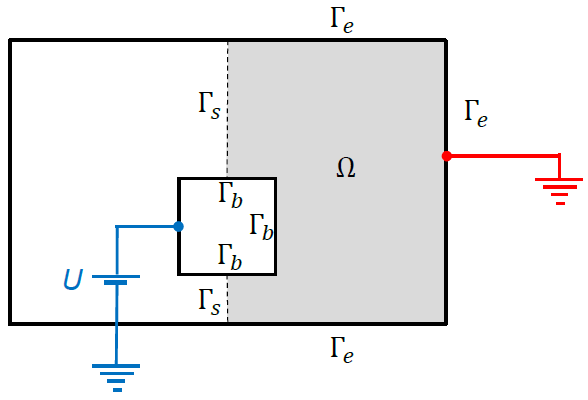
\includegraphics[width=8cm]{images/randbedinung_ES.png}
\end{minipage}
\subsection{Randwertproblem}
\begin{multicols}{2}
\begin{itemize}
	\item $\dfrac{\partial^2\varphi}{\partial x^2} +  \dfrac{\partial^2\varphi}{\partial y^2} + \dfrac{\partial^2\varphi}{\partial z^2}=0 $
	\item $\varphi(x,y,z)=0 \in \Gamma_e$
	\item $\varphi(x,y,z)=0 \in \Gamma_b$
	\item $ \dfrac{\partial\varphi(x,y,z)}{\partial n} = 0 \in \Gamma_s$
\end{itemize}
\end{multicols}
\subsection{Vorgehen}
\begin{enumerate}
	\item Partielle Differentialgleichung 2. Ordnung des Potentials aufstellen (Poisson oder Laplace)
	\item Koordinatentransformation wenn nötig
	\item Vereinfachung der partiellen DGL in eine gewöhnliche DGL 
	\subitem Von welcher Variable hängt das Potential ab
	\item Aufstellen der Randbedingungen
	\subitem Randwerte für Potential und E-Feld
	\item Gewöhnliche DGL 2x integrieren und nach Potential auflösen
	\item Randwerte einsetzen und unbekannte Konstanten bestimmen
\end{enumerate}
\clearpage
\pagebreak

\section{Stationäre Strömungsanalyse (SCD, Stationray Current Distribution)}
Die stationäre Strömungsanalyse wird für die Berechnung des Ersatzwiderstand gebraucht
\subsection{Integralgleichungen}
\begin{tabular}{|p{.30\textwidth} |p{.65\textwidth}|}
	\hline 
	\textbf{Elektrische Stromdichte} \newline
	\tabbild[width=3cm]{images/ElStromdichte} & Die elektrische Stromdichte kennzeichnet wie dicht zusammengedrängt ein elektrischer Strom fliesst. Damit ist auch die Belastung eines Leiters durch den Strom bekannt.\newline
	\[ \vec{J} = \dfrac{dI}{dA}\cdot \vec{n}\qquad [\vec{J}] = \dfrac{A}{m^2} \] \[I = \iint\limits_{(A)}\vec{J}\cdot\vec{dA} \] \\
	\hline
	\textbf{Kontinuitätsgleichung} \newline
	\tabbild[width=3cm]{images/Gauss.png} & Der herausfliessende Strom aus einer geschlossenen Fläche ist gleich der Abnahme der Ladung \newline
		\[ I = -\dfrac{dQ}{dt} = -\dfrac{d}{dt}\iiint\limits_{(V)}\varrho\cdot dV = -\iiint\limits_{(V)}\dfrac{d\varrho}{dt}\cdot dV \]
	 \[ \varoiint\limits_{(A)}\vec{J}\cdot\vec{dA} = -\iiint\limits_{(V)}\dfrac{d\varrho}{dt}\cdot dV \]
	\[ \varoiint\limits_{(A)}\vec{J}\cdot\vec{dA} = 0\] \\
	\hline
	\textbf{Ohmsches Gesetz}\newline
	\tabbild[width=3cm]{images/OhmschesGesetz.png} & 
	\[ J= \sigma \cdot E\]
	\[ R = \varrho\cdot\dfrac{l}{A}\]
	\[ \sigma = \dfrac{1}{\varrho}\]
	\[ G = \sigma\cdot\dfrac{A}{l} \]\\
	\hline
\end{tabular}
\subsection{Differenzialgleichungen der elektrostatischen Analyse}
\begin{multicols}{2}
	\textbf{Stationäre Analyse}\\
	\[\nabla \vec{J} = -\frac{d \rho}{dt}=0\]
	\textbf{Laplace Gleichung}
	\[\dfrac{\partial^2\varphi}{\partial x^2} +  \dfrac{\partial^2\varphi}{\partial y^2} + \dfrac{\partial^2\varphi}{\partial z^2} = \Delta \varphi = 0\]	
\end{multicols}
\clearpage
\pagebreak
\subsection{Randbedingungen}
\begin{minipage}{8cm}
	\begin{itemize}
		\item Der geerdete Rand \[\varphi = 0\]
		\item Der Rand mit bekannten Potential \[ \varphi = U \]
		\item Der Rand der Symmetrie \[ \dfrac{\partial\varphi}{\partial n} = 0\]
		\item Der Rand zwischen zwei Materialien \[\sigma_{1} \cdot \frac{d \varphi_{2}}{dn}=\sigma_{2} \cdot \frac{d \varphi_{1}}{dn}\]
	\end{itemize}
\end{minipage}
\begin{minipage}{8cm}
	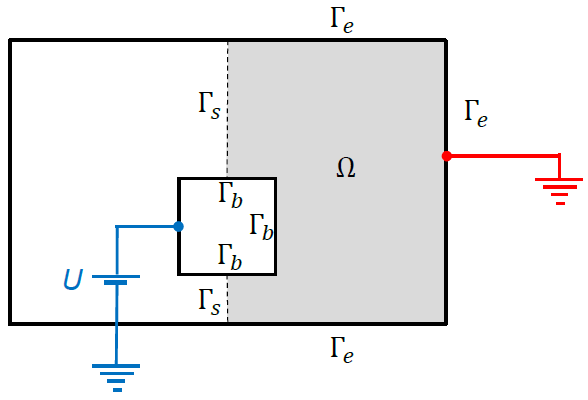
\includegraphics[width=8cm]{images/randbedinung_ES.png}
\end{minipage}
\subsection{Anwendung}
%TODO Beispiel einfügen
\clearpage
\pagebreak
\section{Magnetostatische Analyse (MS, Magnetostatic Analysis)}
Die magnetostatische Analyse basiert auf der gleichmässigen Bewegung des elektrische Stroms. Der elektrische Strom ist über die Zeit konstant. Die magnetostatische Analyse wird für die Berechnung der Ersatzinduktivität von elektrischen Komponenten gebraucht.
\subsection{Integralgleichungen}
\begin{tabular}{|p{.30\textwidth} |p{.65\textwidth}|}
	\hline 
	\textbf{Ampèresches Gesetz} \newline
	{\centering\tabbild[width=4cm]{images/ampgesetz.png}\par} & Das Ampèresche Gesetz definiert die Verteilung des magnetischen Feldes durch eine geschlossene Kurve und dem gesamten Strom durch die entsprechende Fläche
	\[ \oint\limits_{(C)}\vec{H}\cdot\vec{dl} = \iint\limits_{(A)}\vec{J}\cdot\vec{dA}\] \newline
	 \[ \oint\limits_{(C)}\vec{B}\cdot\vec{dl} = \mu_{0}\iint\limits_{(A)}\vec{J}\cdot\vec{dA}  \quad \quad\vec{B}=\mu_{0}\mu_{r}\cdot \vec{H}\]\\
	\hline
	{\centering\textbf{Durchflutungsgesetz}\par}
	& \[ \oint\limits_{(C)}\vec{H}\cdot\vec{dl} = \sum\limits_{k = 1}^{n} I_k = \theta \] 
	 \[ \oint\limits_{(C)}\vec{B}\cdot\vec{dl} = \mu_{0}\sum\limits_{k = 1}^{n} I_k = \theta \]\\
	\hline
	\textbf{Coulombsches Gesetz} \newline
	{\centering\tabbild[width=4cm]{images/quellenfreiheit.png}\par} & Der magnetische Fluss durch eine geschlossene Fläche ist immer Null. Somit sind die magnetische Feldlinien immer geschlossen. Es gibt keine magnetische Monopole. Das magnetische Feld ist quellenfrei \newline
	\[ \oiint\limits_{(A)}\vec{B}\cdot\vec{dA} = 0\]\\
	\hline
\end{tabular}
\clearpage
\pagebreak
\subsection{Differenzialgleichungen der magnetostatischen Analyse}
\begin{tabular}{|p{.45\textwidth} |p{.45\textwidth}|}
	\hline
	\textbf{Differenzialgleichung der Durchflutung}\newline
	\[\rotation \vec{H}=\nabla \times \vec{H}=\vec{J}\]
	\[\rotation \vec{B}=\nabla \times \vec{B}=\mu_{0}\vec{J}\]&
	\textbf{Poissongleichung}\newline
	Die obige Gleichung wird mit Umweg über das Vektorpotential A des Magnetfeldes gelöst
	\[\nabla \times \vec{A}=\vec{B} \quad \nabla\cdot \vec{A} =0\]	
	\[\Delta\vec{A}=-\mu_{0}\vec{J}\]\\
	\hline
\end{tabular}
\subsection{Randbedingungen}
\begin{itemize}
	\item Magnetische Isolierung $\vec{n} \times \vec{A} =0$
	\item Der Rand zwischen zwei Materialien $\vec{n} \times \vec{A_{1}}=\vec{n} \times \vec{A_{2}}$
\end{itemize}
\subsection{Randwertproblem}
\begin{minipage}{8cm}
	\begin{itemize}
		\item $\Delta\vec{A}=-\mu_{0}\vec{J}$
		\item $\vec{n} \times \vec{A} =0$
	\end{itemize}	
\end{minipage}
\begin{minipage}{8cm}
	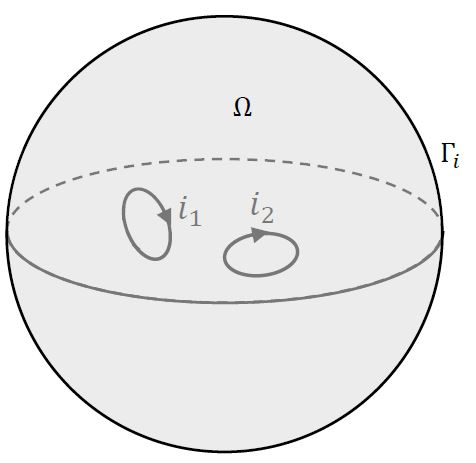
\includegraphics[width=4cm]{images/Randwertproblem.jpg}
\end{minipage}
\clearpage
\pagebreak
\section{Magnetoquasistatische Analyse (MQS, Magnetoquasistatic Analysis)}
%TODO Magnetoquasistatische Analyse
\subsection{Integralgleichungen}
\begin{tabular}{|p{.30\textwidth} |p{.65\textwidth}|}

\end{tabular}
\subsection{Differenzialgleichungen der magnetoquasostatischen Analyse}
\subsection{Randbedingungen}
\subsection{Anwendung}
\clearpage
\pagebreak
\section{Maxwell Gleichungen}
\subsection{Maxwell Gleichungen}
\begin{longtable}{|p{.08\textwidth}|p{.25\textwidth} |p{.25\textwidth}|p{.30\textwidth}| }
	\hline
	\textbf{Gesetz}&\textbf{Differentialform} &\textbf{Differentialform} &\textbf{Integralform}\\
	&1. Art & 2. Art &\\
	\hline
	1.&$\divergenz \vec{D}=\nabla \cdot \vec{D}= \rho$ & $\divergenz \vec{E}= \frac{\rho}{\epsilon}$&$\oint\limits_{\partial V}\vec{D}\cdot d\vec{A}=\int\int\int\limits_{V}\rho \cdot dV=Q$\\
	\hline
	2.&$\divergenz \vec{B}=\nabla \cdot \vec{B}=0$&$\divergenz \vec{H}=\nabla \cdot \vec{H}=0 $&$\oint\limits_{\partial V}\vec{B}\cdot d\vec{A}=0$\\
	\hline
	3.&$\rotation \vec{E}=\nabla \times \vec{E}=-\frac{\partial B}{\partial t}$&$\rotation \vec{E}=\nabla \times \vec{E}=-\mu \frac{\partial H}{\partial t}$&$\oint\limits_{\partial A}\vec{E}\cdot ds=-\iint\limits_{A}\frac{\partial B}{\partial t}\cdot dA$\\
	\hline
	4.&$\rotation\vec{B}=\nabla\times\vec{B}=\mu_0 (J+\frac{\partial D}{\partial t})$&$\rotation \vec{H}=\nabla \times \vec{H}=\sigma\vec{E}+\epsilon \frac{\partial E}{\partial t}$&$\oint\limits_{\partial A} \vec{H}\cdot ds$\\
	\hline
\end{longtable}
\subsection{Erstes Maxwell-Gesetz}
Gausssches Gesetz für Elektrische Felder\\
\begin{tabular}{p{.45\textwidth} p{.45\textwidth}}
	\textbf{Differentialform}&\textbf{Integralform}\\
	Das E-Feld ist ein Quellenfeld. Die Ladung ist die Quelle des elektrischen Feldes. & Der elektrische Fuss durch die geschlossene Oberfläche eines Volumen ist direkt proportional zur elektrischen Ladung in seinem inneren. \\
\end{tabular}
\subsection{Zweites Maxwell-Gesetz}
Gausssches Gesetz für Magnetische Felder\\
\begin{tabular}{p{.45\textwidth} p{.45\textwidth}}
	\textbf{Differentialform}&\textbf{Integralform}\\
	Das B-Feld ist quellenfrei. Es gibt keine magnetische Monopole (Magnet welcher nur ein Pol hat).& Der magnetische Fluss durch die Oberfläche eines Volumen ist gleich der magnetischen Ladung in seinem inneren, nämlich Null.\\
\end{tabular}
\subsection{Drittes Maxwell-Gesetz}
Induktionsgesetz\\
\begin{tabular}{p{.45\textwidth} p{.45\textwidth}}
	\textbf{Differentialform}&\textbf{Integralform}\\
	Jede Änderung des B-Feldes führt zu einem elektrischen Gegenfeld. Die Wirbel des elektrischen Feldes sind von der zeitlichen Änderung der magnetischen Flussdichte abhängig (Induktionsgesetz). & Die elektrische Zirkulation (Umlaufintegral eines Vektorfeldes über  einen geschlossenen Weg) über eine Kurve einer Fläche ist gleich der negativen Änderung des magnetischen Flusses durch die Fläche.\\
\end{tabular}
\subsection{Viertes Maxwell-Gesetz}
Durchflutungsgesetz\\
\begin{tabular}{p{.45\textwidth} p{.45\textwidth}}
	\textbf{Differentialform}&\textbf{Integralform}\\
	Die Wirbel des Magnetfeldes hängen von der Stromdichte und von der elektrischen Flussdichte ab. Die zeitliche Änderung der Flussdichte wird als Verschiebungsstromdichte bezeichnet (Durchflutungsgesetz)& Die magnetische Zirkulation über eine Kurve einer Fläche ist gleich der Summe aus dem Leitungsstrom und der zeitlichen Änderung des Flusses durch die Fläche. \\
\end{tabular}
\clearpage
\pagebreak

\subsection{Elektromagnetische Wellengleichung}
Eine Elektromagnetische Welle erfüllt immer die nachfolgenden Gleichung. Anhand dieser ist ersichtlich das für die Welle keine Ladung nötig ist sonder das E-Feld und das B-Feld beschäftigen sich mit sich selber und weil ein E-Feld und B-Feld nach sich zieht und umgekehrt. Damit breitet sich die Welle aus. \\
\begin{minipage}{8cm}
	\[\begin{matrix}
	\divergenz \vec{E}=0\\
	\divergenz \vec{B}=0\\
	\rotation \vec{H}=\epsilon_{0}\mu_{0} \frac{\partial \vec{E}}{\partial t}\\
	\rotation \vec{B}=-\dfrac{\partial \vec{B}}{\partial t}\\
	\rotation \vec{E}=-\mu_{0}\dfrac{\partial \vec{H}}{\partial t}
	\end{matrix}\]
\end{minipage}
\begin{minipage}{8cm}
	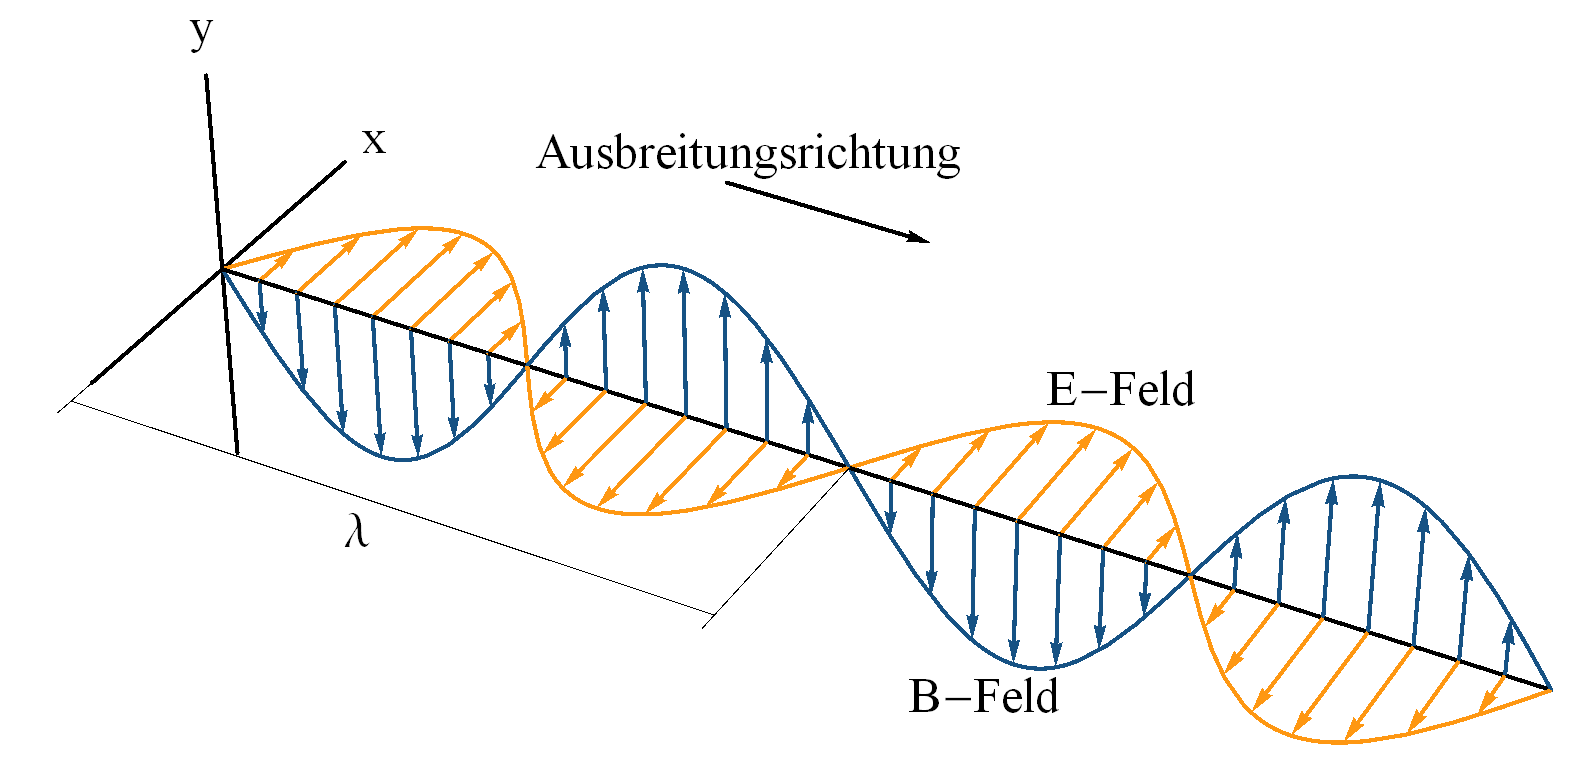
\includegraphics[width=8cm]{images/EMWelle.jpg}
\end{minipage}

\begin{tabular}{p{.45\textwidth} p{.45\textwidth}}
	{\hspace{-2.5cm}\centering\textbf{Magnetisches Feld}\par}&{\hspace{-2.5cm}\centering\textbf{Elektrisches Feld}\par}\\[-1.5cm]
	\[\Delta\vec{H}-\mu\sigma\frac{\partial \vec{H}}{\partial t}-\mu\epsilon\frac{\partial^{2}\vec{H}}{\partial t^{2}}=0\]&	\[\Delta\vec{E}-\mu\sigma\frac{\partial \vec{E}}{\partial t}-\mu\epsilon\frac{\partial^{2}\vec{E}}{\partial t^{2}}=0\]  \\
\end{tabular}
\subsection{Randbedingungen}
\begin{itemize}
	\item Am Rand zwischen zwei Materialien $H_{t1}=H_{t2}$
	\item Am Rand zwischen zwei Materialien $B_{n1}=B_{n2}$
	\item Am Rand zwischen zwei Materialien $E_{t1}=E_{t2}$
	\item Am Rand zwischen zwei Materialien $D_{n1}=D_{n2}$
\end{itemize}
\subsection{Randwertproblem}
\begin{minipage}{9cm}
	\begin{itemize}
		\item Zeitbereich: $\Delta\vec{H}-\mu\sigma\frac{\partial \vec{H}}{\partial t}-\mu\epsilon\frac{\partial^{2}\vec{H}}{\partial t^{2}}=0$
		\item Frequenzbereich: $\Delta \vec{H}-\imaginär\omega\mu\sigma\vec{H}+\omega^{2}\mu\epsilon\vec{H}=0$
		\item Sobald eine Welle auf einen Rand trifft wird immer ein Teil reflektiert und der andere geht durch
	\end{itemize}	
\end{minipage}
\begin{minipage}{8cm}
	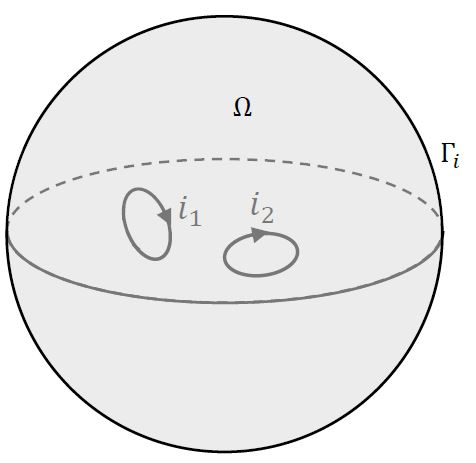
\includegraphics[width=4cm]{images/Randwertproblem.jpg}
\end{minipage}
\subsection{Vorgehen}
	\begin{enumerate}
		\item Partielle Differentialgleichung 2. Ordnung der Welle aufstellen (Elektrisch oder Magnetisch)
		\item In Frequenzbereich transformieren (Annahme sinusförmige Anregung)
		\subitem $\dfrac{\partial \vec{F}}{\partial t}= j\omega F $
		\item Differentialgleichung vereinfachen
		\item Aufstellen der Randbedingungen
		\subitem Randwerte für E-Feld und H-Feld
		\item Wellengleichung mittels Charakteristischem Polynom lösen da Homogen
		\item Bestimmung der Unbekannten Amplituden mittels den Randbedingungen
	\end{enumerate}
\clearpage
\pagebreak
\subsection{Grundlagen zu den Maxwellgleichungen}
Die Maxwell Gleichungen beschreiben, dass die Feldlinien eines sich ändernden Magnetfeldes von ringförmigen elektrischen Feldlinien umgeben sind, auch ohne Vorhandensein von elektrischen Leitern. Darauf die Theorie der elektromagnetischen Wellen auf. Grundlage der Maxwellschen Theorie sind die Maxwellschen Gleichungen. Es zeigt sich, dass die Lösungen der Gleichungen elektromagnetische Wellen beschreiben.\\
\vspace{0.2cm}\\
\renewcommand{\arraystretch}{1.2}
\begin{tabular}{|p{.45\textwidth} |p{.45\textwidth}|}
	\hline
	\textbf{Elektrische Kraft}\newline
	\[\vec{F}=q\cdot \vec{E}\]&
	\textbf{Magnetische Kraft}\newline
	\[\vec{F}=q\cdot(\vec{v}\times \vec{B})\]\\
	\hline
	\textbf{Elektrische Raumladungsdichte}\newline
	Sagt aus wieviel Ladung sich im Raum befindet\newline
	\[ \rho  = \frac{Q}{V}\]&
	\textbf{Elektrische Stromdichte}\newline
	Sagt aus wie die Ladung rämumlich verteilt ist\newline
	\[\vec{J}=\rho \cdot \vec{v}\]\\
	\hline
	\textbf{Wellenimpedanz der Luft}\newline
	\[Z_{0}=\sqrt{\frac{\mu_{0}}{\epsilon_{0}}} \]&
	\textbf{Wellenimpedanz eines Isolators}\newline
	\[Z=\sqrt{\frac{\mu_{0}}{\epsilon}} \]\\
	\hline
	\textbf{Kapazität}\newline
	\[C=\frac{Q}{U} \] &
	\textbf{Induktivität}\newline
	\[L=\frac{N\cdot \Phi }{I} \]\\
	\hline
	\textbf{Magnetische Energie}\newline
	\[W= \frac{1}{2}\cdot L \cdot I^{2}\]&
	\textbf{Elektrische Energie}\newline
	\[W= \frac{1}{2}\cdot C \cdot U^{2}=\frac{1}{2}\cdot Q\cdot U \]\\
	\hline
	\textbf{Lichtgeschwindigkeit} \newline
	\[ c = \dfrac{1}{\sqrt{\mu_0\varepsilon_0}}\] & 
	\textbf{Skin-Tiefe}\newline 
	\[ \delta = \sqrt{\dfrac{2}{\omega\mu_0\sigma}}\] \\
	\hline
\end{tabular}

\input{sections/fem}
\section{Anwendungen}
\subsection{Dieelektrische Berechnung von Hochspannungsgeräten}
\begin{itemize}
	\item Das elektrische Feld einer geometrischen Anordnung hängt von den Abständen zwischen den Elektroden und den geerdeten Flächen ab.
	\item Die Felderhöhung entsteht an scharfen Ecken und Kanten
	\item Abrundung dieser scharfen Stellen verringert das elektrische Feld
	\item Falls eine Abrundung nicht möglich ist, wird eine elektrische Abschirmung eingebaut
\end{itemize}
\subsection{Wirbelströme in Transformatoren}
\begin{itemize}
	\item Das magnetische Streufeld eines Transformators induziert in den Wicklungen Wirbelströme
	\item Diese Wirbelströme sorgen für eine zusätzliche Erwärmung der Bauteile im Trafo
	\item Die Wirbelströme können nur über Simulationen berechnet werden. 
\end{itemize}
\subsection{Elektromagnetische Analyse von Elektrischen Maschinen}
\begin{itemize}
	\item Das magnetische Feld wird durch die Statorwicklung erzeugt
	\item Die Leiter im Rotor werden vom magnetischen Feld durchflossen. Durch die magnetischen Kräfte des Feldes wird das Drehmoment erzeugt. 
	\item Durch Simulationen können die Kennwerte der elektrischen Maschine berechnet werden
\end{itemize}
\subsection{Eigenwertanalyse von Wellenleitern}
\begin{itemize}
	\item Das Design von Wellenleitern basiert auf der Eigenwertanalyse
	\item Eigenwertanalyse: Eigenwert (Wellenausbreitungskonstante), Eigenvektor (Feldverteilung für gegebene Frequenz)
\end{itemize}
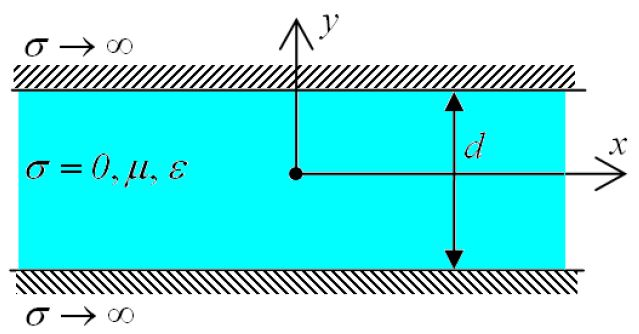
\includegraphics[width=6cm]{images/Wellen.jpg}\\
\begin{tabular}{|p{0.45\textwidth} |p{0.45\textwidth}|}
	\hline
	\textbf{Wellengleichung}\newline
	$\dfrac{d^2E}{dy^2}+(\omega^2-\mu\epsilon-\gamma^2)E_z=0 $&
	\textbf{Lösung der Wellengleichung}\newline
	$E= \underbrace{A\cos(k\cdot y)\cdot \euler^{-j\frac{\gamma}{y}}}_{\text{Even Modes}} + \underbrace{B\sin(k\cdot y)\cdot \euler^{-j\frac{\gamma}{x}}}_{\text{Odd Modes}} $ \\
	\hline
	\textbf{Even Mode}\newline
	$\cos(k \cdot \frac{\pm d}{2}) \rightarrow k=\frac{2n+1}{d} \cdot \pi $\newline
	\tabbild[width=6cm]{images/Even.jpg}
	&
	\textbf{Odd Mode}\newline
	$\sin(k \cdot \frac{\pm k}{2}) \rightarrow k=\frac{2n}{d} \cdot \pi $\newline
	\tabbild[width=6cm]{images/Odd.jpg}\\
	\hline
\end{tabular}
\vspace{0.5cm}\\
\subsubsection{Eigenwertanalyse Homogener Wellenleiter}
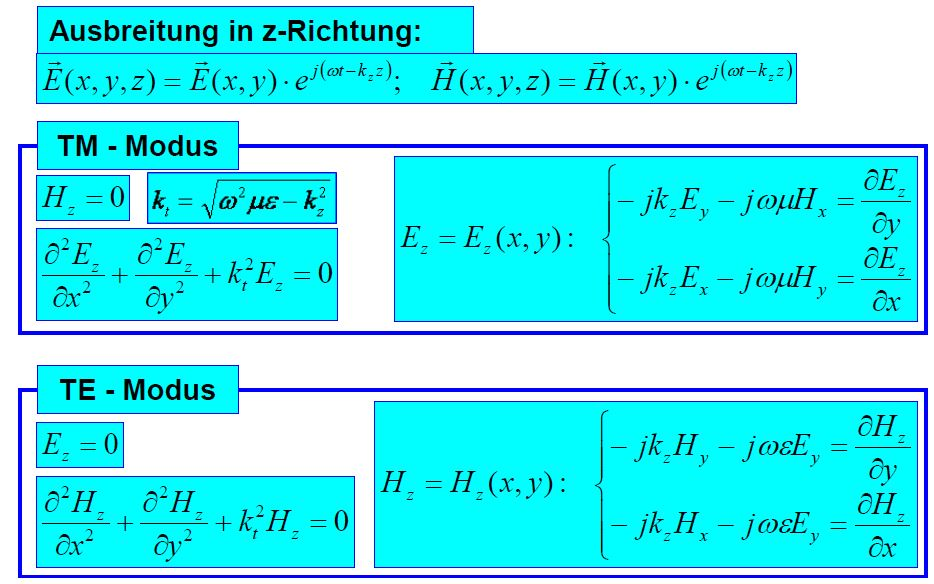
\includegraphics[width=0.8\linewidth]{images/Eigenwertanalyse.jpg}
\end{document}
